%\documentclass[slidestop,mathserif]{beamer}
\documentclass{beamer}
%\documentclass{beamer}
%\definecolor{SKIcolor}{rgb}{221,54,49}
%\usecolortheme[named=SKIcolor]{structure}
%\usepackage{beamerthemePostech}
%\usetheme{AnnArbor}
\usetheme{Madrid}
\usepackage{arev}
\usepackage{xcolor}
\usepackage{color}
%\usepackage{subfigure}
\usepackage{multirow}
\usepackage{amsmath}
\usepackage{amsthm}
\usepackage{amsfonts}
\usepackage{hyperref}
\usepackage{mathrsfs}
\usepackage[listings,theorems]{tcolorbox}
\usepackage{algorithm2e}
\usepackage{algpseudocode}
\usepackage{mathtools}
\usepackage{adjustbox}
\usepackage{chngcntr}
\usepackage{kotex}
\usepackage{booktabs}
\usepackage{subfig}
\usepackage{makecell}
\usepackage{forest}
\usepackage[flushleft]{threeparttable}
\def\nine{\fontsize{9pt}{9pt}\selectfont}
\def\eight{\fontsize{8pt}{8pt}\selectfont}
\def\seven{\fontsize{7pt}{7pt}\selectfont}
\def\ttiny{\fontsize{6pt}{6pt}\selectfont}
\def\Tiny{\fontsize{5pt}{5pt}\selectfont}

%% Package, Library, abbreviate terms
\newcommand{\siplibtwo}{\textsf{SIPLIB 2.0}}
\newcommand{\siplib}{\textsf{SIPLIB}}
\newcommand{\miplib}{\textsf{MIPLIB 2010}}
\newcommand{\smps}{\textsf{SMPS}}
\newcommand{\mps}{\textsf{MPS}}
\newcommand{\mpsx}{\textsf{MPSX}}
\newcommand{\jump}{\textsf{JuMP}}
\newcommand{\structjump}{\textsf{StructJuMP}}

% Problems
\newcommand{\airlift}{\textsf{AIRLIFT}}
\newcommand{\chem}{\textsf{CHEM}}
\newcommand{\dcap}{\textsf{DCAP}}
\newcommand{\sdcp}{\textsf{SDCP}}
\newcommand{\mptsps}{\textsf{MPTSPs}}
\newcommand{\sizes}{\textsf{SIZES}}
\newcommand{\smkp}{\textsf{SMKP}}
\newcommand{\sslp}{\textsf{SSLP}}
\newcommand{\suc}{\textsf{SUC}}
\newcommand{\cargo}{\textsf{CARGO}}
\newcommand{\phone}{\textsf{PHONE}}

% Solvers
\newcommand{\dsp}{\textsf{DSP}}
\newcommand{\pysp}{\textsf{PySP}}
\newcommand{\pyomo}{\textsf{Pyomo}}
\newcommand{\cplex}{\textsf{CPLEX}}
\newcommand{\scip}{\textsf{SCIP}}
\newcommand{\pipssbb}{\textsf{PIPS-SBB}}

%% Programming languages
\newcommand{\julia}{\texttt{Julia}}
\newcommand{\python}{\texttt{Python}}
\newcommand{\clang}{\texttt{C}}
\newcommand{\cpp}{\texttt{C++}}
\newcommand{\matlab}{\texttt{MATLAB}}

%% Siplib.jl related terms
\newcommand{\jumpmodel}{\texttt{JuMP.Model}}
\newcommand{\siplibjl}{\texttt{Siplib.jl}}

\setcounter{tocdepth}{2}

% for Siplib.jl tree
\definecolor{folderbg}{RGB}{124,166,198}
\definecolor{folderborder}{RGB}{110,144,169}
\def\Size{4pt}
\tikzset{
	folder/.pic={
		\filldraw[draw=folderborder,top color=folderbg!50,bottom color=folderbg]
		(-1.05*\Size,0.2\Size+5pt) rectangle ++(.75*\Size,-0.2\Size-5pt);  
		\filldraw[draw=folderborder,top color=folderbg!50,bottom color=folderbg]
		(-1.15*\Size,-\Size) rectangle (1.15*\Size,\Size);
	}
}

% for Julia script
\lstdefinelanguage{julia}
{
	sensitive=true,	
	basicstyle=\ttfamily\scriptsize,
	columns=fullflexible, % make sure to use fixed-width font, CM typewriter is NOT fixed width
	numbers=left, 
	numberstyle=\small\ttfamily\color{Gray},
	stepnumber=0,              
	numbersep=10pt, 
	numberfirstline=true, 
	numberblanklines=true, 
	tabsize=4,
	lineskip=-1.5pt,
	extendedchars=true,
	breaklines=true,        
	keywordstyle=\color{Blue}\bfseries,
	identifierstyle=, % using emph or index keywords
	commentstyle=\sffamily\color{OliveGreen},
	stringstyle=\color{Maroon},
	showstringspaces=false,
	showtabs=false,
	upquote=false,
	keywordsprefix=\@,
	keywords={exit,whos,edit,load,is,isa,isequal,typeof,tuple,ntuple,uid,hash,finalizer,convert,promote,
		subtype,typemin,typemax,realmin,realmax,sizeof,eps,promote_type,method_exists,applicable,
		invoke,dlopen,dlsym,system,error,throw,assert,new,Inf,Nan,pi,im,begin,while,for,in,return,
		break,continue,macro,quote,let,if,elseif,else,try,catch,end,bitstype,ccall,do,using,module,
		import,export,importall,baremodule,immutable,local,global,const,Bool,Int,Int8,Int16,Int32,
		Int64,Uint,Uint8,Uint16,Uint32,Uint64,Float32,Float64,Complex64,Complex128,String,Symbol,Any,Nothing,None,
		function,type,typealias,abstract,struct, mutable},
	comment=[l]{\#},
	%morecomment=[s]{#=}{=#},
	morestring=[d]\',
	morestring=[b]\",
}

%\newtheorem{lemma}{Lemma}
\newtheorem{proposition}{Proposition}
\newcommand{\argmin}{\arg\!\min}
\newcommand{\argmax}{\arg\!\max}
\DeclarePairedDelimiter{\ceil}{\lceil}{\rceil}
\DeclarePairedDelimiter{\floor}{\lfloor}{\rfloor}
\DeclareMathOperator*{\PP}{\mathbb{P}}
\DeclareMathOperator*{\EE}{\mathbb{E}}
\SetKwRepeat{Do}{do}{while}    
\setlength\abovecaptionskip{-3pt}
\setbeamertemplate{footline}[frame number]
\counterwithin*{equation}{section}      %식번호를 섹션이 바뀔때마다 초기화하라 \usepackage{chngcntr} 필요
\counterwithin*{equation}{subsection}

% enumerate 번호 기억
\newcounter{savedenum}
\newcommand*{\saveenum}{\setcounter{savedenum}{\theenumi}}
\newcommand*{\resume}{\setcounter{enumi}{\thesavedenum}}

%\setbeamercovered{transparent}
\setbeamercovered{invisible}

%\fboxsep=10mm%padding thickness
\fboxrule=0.7pt%border thickness

% Contents에 한글 표시
\hypersetup{
	unicode=true, %
}
\title{\textbf{SIPLIB 2.0}}
\subtitle{Stochastic Integer Programming Library version 2}

\author{\underline{Yongkyu Cho}\inst{1}\inst{2} \and Kibaek Kim\inst{2} \\ \and James Luedtke\inst{3} \and Jeffrey Linderoth\inst{3}}
\institute[] % (optional, but mostly needed)
{
	\inst{1}%
	Department of Industrial and Management Engineering\\
	Pohang University of Science and Technology
	\and
	\inst{2}%
	Mathematics and Computer Science Division\\
	Argonne National Laboratory
	\and
	\inst{3}%
	Department of Industrial and Systems Engineering\\
	University of Wisconsin-Madison
}
\date{INFORMS Annual Meeting 2018}


\begin{document}
	
	\tcbset{%
		noparskip,
		colback=white, %background color of the box
		colframe=black, %color of frame and title background
		coltext=black, %color of body text
		coltitle=white, %color of title text 
		fonttitle=\bfseries,
	}
	
	\setbeamercovered{transparent=30}
	\begin{frame}
	\titlepage
\end{frame}

\frame{
	\frametitle{Contents}
	\tableofcontents[hideothersubsections]
	\setcounter{tocdepth}{2}
}

\section{Overview}
\begin{frame}<beamer>{Contents}
\tableofcontents[currentsection,currentsubsection,hideothersubsections]
\end{frame}	

\begin{frame}{What is \siplib?}
\footnote{\tiny Available at: \href{https://www2.isye.gatech.edu/~sahmed/siplib/}{https://www2.isye.gatech.edu/~sahmed/siplib/}}{\siplib}: A Stochastic Integer Programming Test Problem Library
\begin{itemize}
\item \siplib\ is a collection of test problems to facilitate \textcolor{blue}{computational and algorithmic research} in stochastic integer programming (SIP).
\item The test problem data is provided in the \textcolor{blue}{standard \smps\ format} unless otherwise mentioned.
\item Where available, \textcolor{blue}{information on the underlying problem formulation} and \textcolor{blue}{known solution} is also included.
\end{itemize}
\end{frame}

\begin{frame}{Limitation of the former \siplib}
\begin{enumerate}
\item Number of the instances
\begin{itemize}
\item Researchers in this field need more test set.
\end{itemize}
\item Variation of problem types
\begin{itemize}
\item Provides only 5 different variations in terms of variable types: continuous, binary, integer.
\end{itemize}
\item Contribution rule
\begin{itemize}
\item Different problem provides different information.
\item For some problems, only limited information is available.
\end{itemize}
\end{enumerate}
\end{frame}

\begin{frame}{Contribution of \siplibtwo}
\textbf{\siplibtwo} provides
\begin{itemize}
\item \textcolor{blue}{more instances} accompanied with \textcolor{blue}{analytic \& computational information}
\item \textcolor{blue}{a \julia\ package} to support
\begin{itemize}
\item generating new instances in SMPS format
\item analyzing the instances (size, sparsity)
\item solving the instances to get some known bounds
\end{itemize}
\item \textcolor{blue}{all the details} about the problems
\begin{itemize}
\item formulation, deterministic \& random parameters
\item parameterized modeling scripts
\end{itemize}
\end{itemize}
\end{frame}

\section{Stochastic Integer Programming}

\begin{frame}<beamer>{Contents}
\tableofcontents[currentsection,currentsubsection,hideothersubsections]
\end{frame}

\begin{frame}{Problem of interest}
\textbf{{Two-stage Stochastic Integer Programming (TSSIP)}}
\begin{itemize}
\item Considers only \textcolor{blue}{two stages}.
\begin{itemize}
\item \textcolor{blue}{Present} (first-stage) and \textcolor{blue}{Future} (second-stage)
\end{itemize} 
\item First-stage decision must be made \textcolor{blue}{for now}.
\item Second-stage decision can be made \textcolor{blue}{after the future is realized} (called \textit{recourse} action).
\item First-stage decision affects the second-stage decision as well.
\end{itemize}
\end{frame}

\begin{frame}[shrink=15]{Mathematical formulation}
\textbf{TSSIP:}
\begin{align}
\min_{x\in X}{\left\{c^\top x + \mathcal{Q}(x):\ Ax\ge b\right\}} \label{eq:SIP_1}
\end{align}
\vspace{-0.4cm}
\begin{itemize}
\item $X\subseteq \mathbb{R}^{n_1-k_1}\times\mathbb{Z}^{k_1}$
\item $c\in\mathbb{R}^{n_1}$
\item $A\in\mathbb{R}^{m_1\times n_1}$
\item $b\in\mathbb{R}^{m_1}$
\item $\mathcal{Q}(x):=\EE_{\pmb{\xi}}[Q(x,\pmb{\xi})]$ (expected recourse function)
\item $\pmb{\xi}$ is a random element defined on a probability triple $(\Xi, \mathcal{F},\PP)$
\end{itemize}
\vspace{0.4cm}
\textbf{Recourse function} $Q(\cdot,\cdot)$:
\begin{align}
Q(x,\xi_s):=\min_{y\in Y}\left\{q(\xi_s)^\top y : W(\xi_s)y\ge h(\xi_s)-T(\xi_s)x\right\}
\end{align}
\vspace{-0.4cm}
\begin{itemize}
\item $\xi_s$ is a realized random element (called \textit{scenario})
\item $Y\subseteq\mathbb{R}^{n_2-k_2}\times\mathbb{Z}^{k_2}$
\item $q(\xi_s)\in\mathbb{R}^{n_2}$
\item $W(\xi_s)\in\mathbb{R}^{m_2\times n_2}$
\item $h(\xi_s)\in\mathbb{R}^{m_2}$
\item $T(\xi_s)\in\mathbb{R}^{m_2\times n_1}$
\end{itemize}		
\end{frame}

\begin{frame}{Mathematical formulation}
\textbf{Deterministic Equivalent Form} (DEF):
\begin{subequations}\label{sip:ef}
\begin{align}
\min_{x,\mathrm{y}}\ &c^{\top}x + \sum_{s=1}^{r}\PP(s) (q_s^{\top}y_s) \label{ef:obj}\\ 
\mathrm{s.t.}\ &Ax\ge b,  \label{ef:b}\\
&T_s x+W_s y_s\ge h_s,\quad\forall s\in\{1,\ldots,r\}, \label{ef:c} \\
&x\in X, \label{ef:d} \\
&y_s \in Y,\quad\forall s\in\{1,\ldots,r\}. \label{ef:e}
\end{align}
\end{subequations}
\vspace{-0.4cm}
\begin{itemize}
\item $\mathrm{y}:=\{y_1,y_2,\ldots,y_r\}$
\item $q_s:=q(\xi_s)$
\item $W_s:=W(\xi_s)$
\item $h_s:=h(\xi_s)$
\item $T_s:=T(\xi_s)$
\end{itemize}
\end{frame}

\begin{frame}{DEF: Block-diagonal structure}
\begin{figure}
\begin{center}
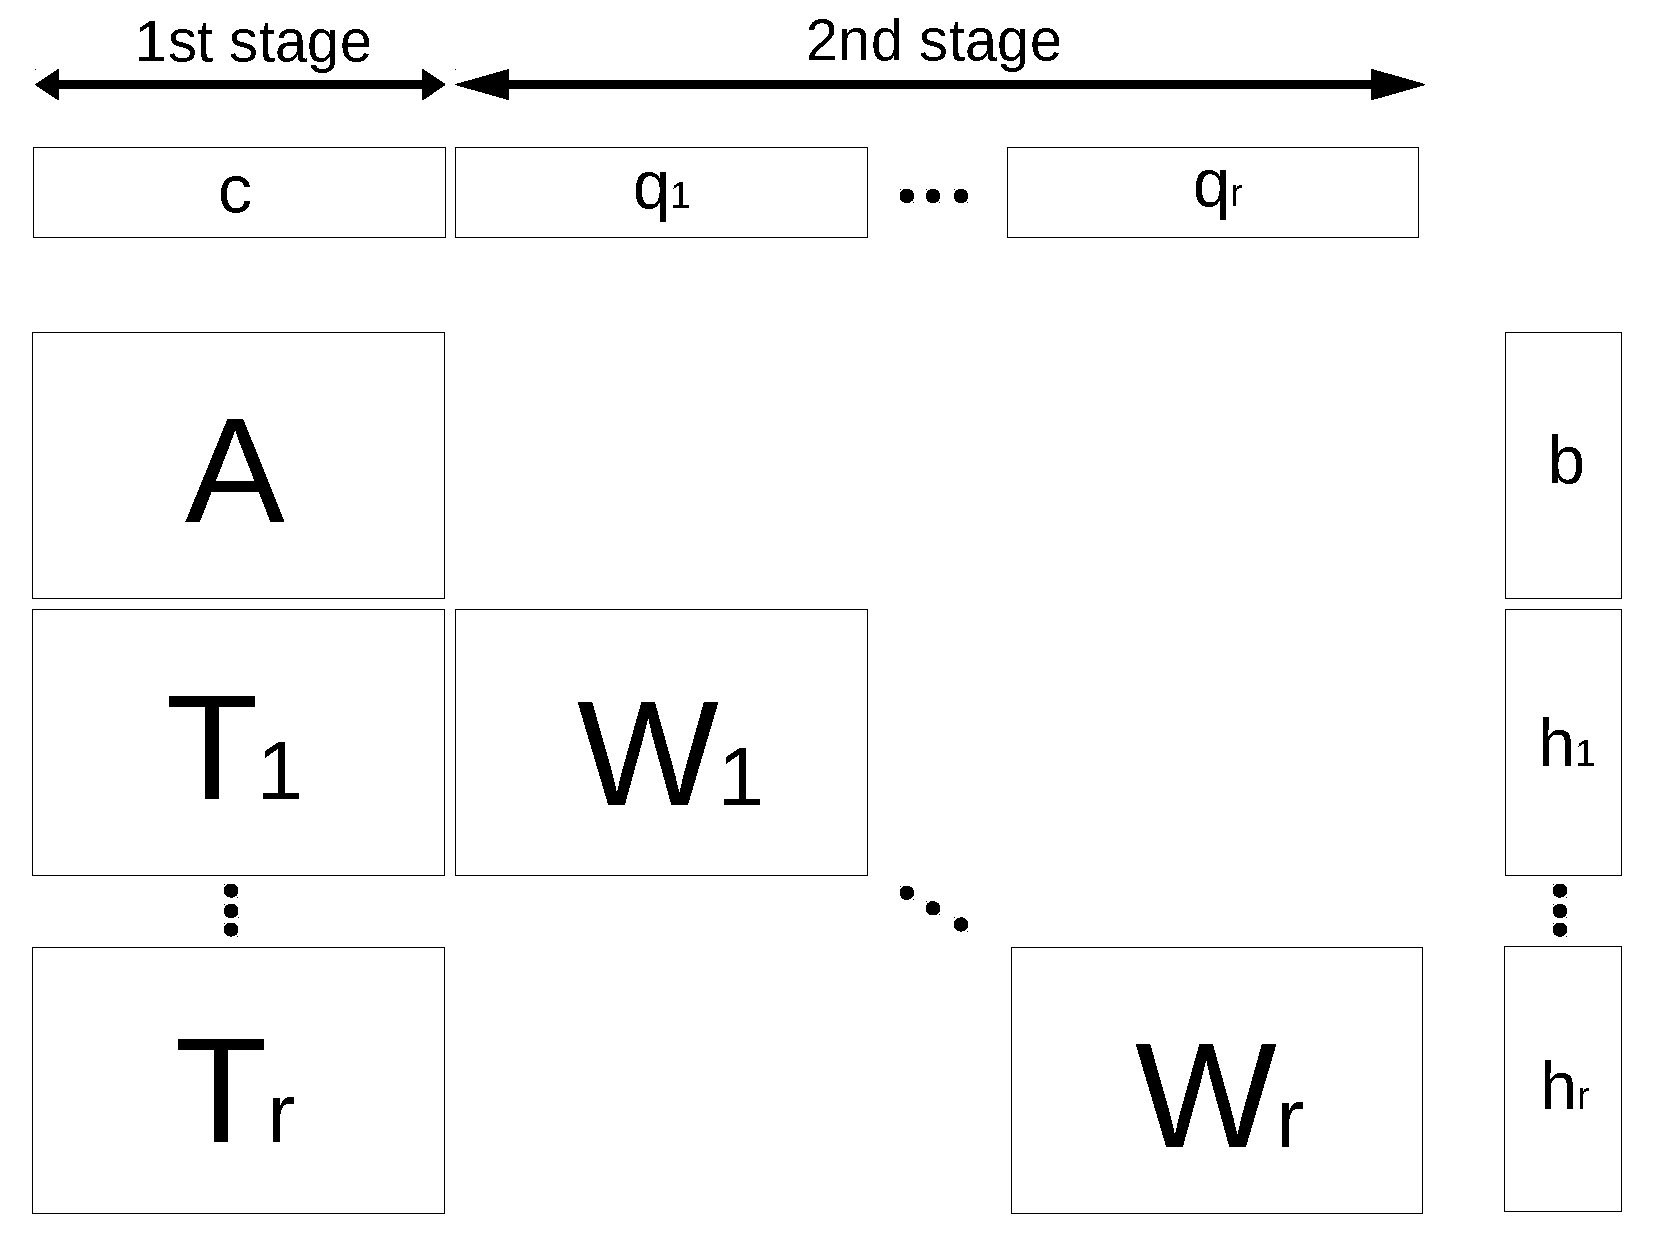
\includegraphics[width=0.9\textwidth]{stagewise_sparsity_slide}
\end{center}
\end{figure}
\end{frame}

\begin{frame}{DEF: Block-diagonal structure}
\vspace{-0.5cm}
\begin{figure}
\centering
\subfloat[][AIRLIFT\_3]
{
\centering
\includegraphics[width=0.35\linewidth]{AIRLIFT_3}
}
~
\subfloat[][CHEM\_3]
{
\centering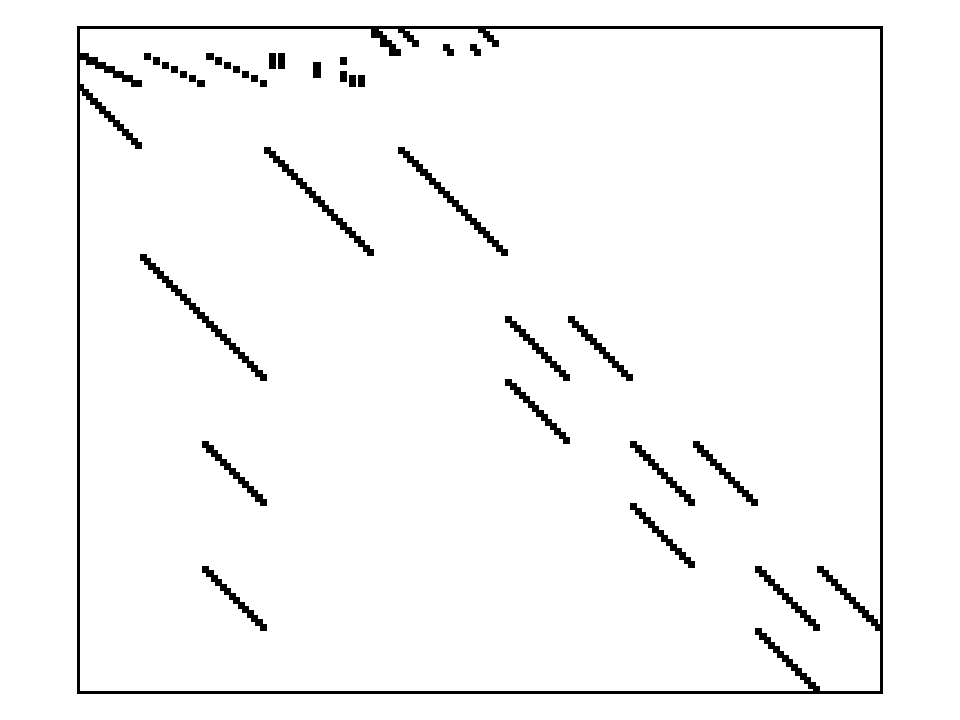
\includegraphics[width=0.35\linewidth]{CHEM_3}
}
\vspace{-0.05cm}
\subfloat[][DCAP\_3\_3\_3\_3]
{
\centering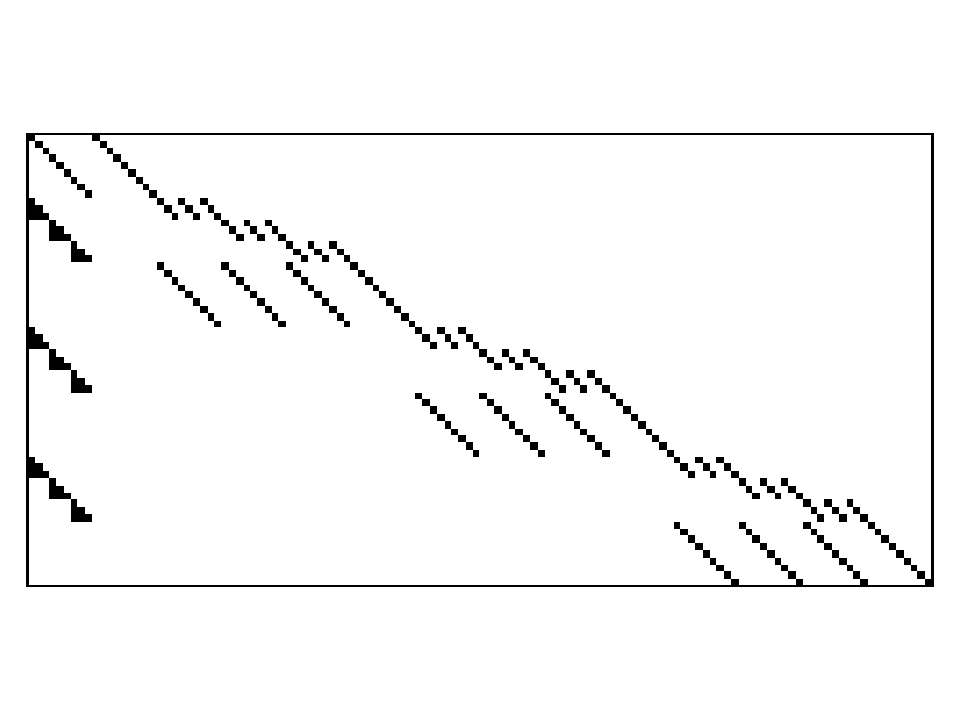
\includegraphics[width=0.35\linewidth]{DCAP_3_3_3_3}
}
~
\subfloat[][SSLP\_5\_10\_3]
{
\centering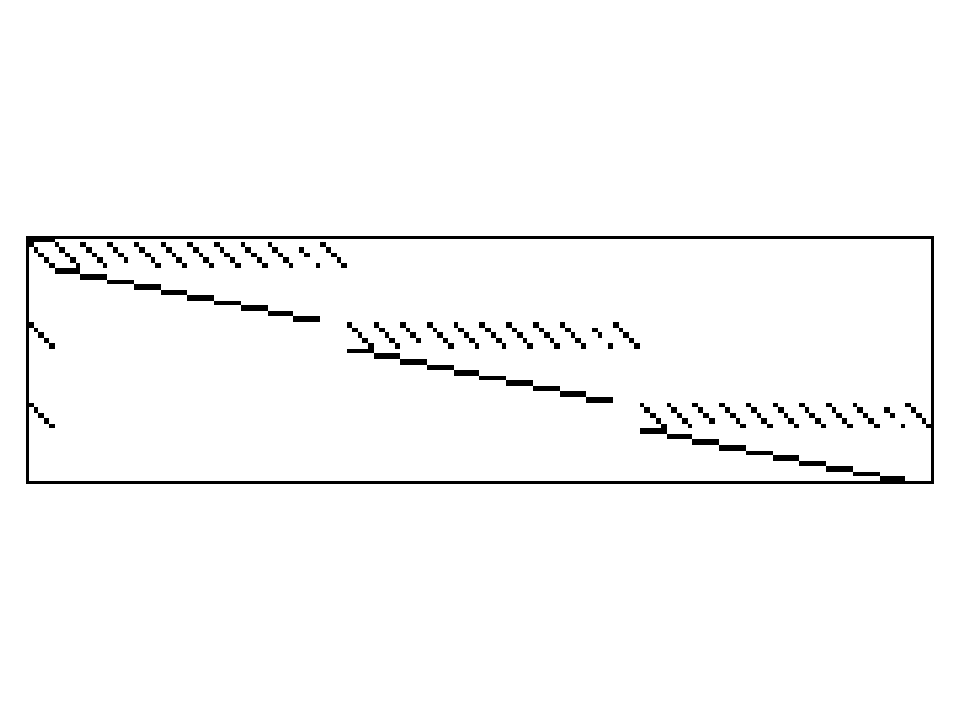
\includegraphics[width=0.35\linewidth]{SSLP_5_10_3}
}
\vspace{0.5cm}
\caption{Example: Repeated sparsity patterns in DEF}
%\label{data3}
\end{figure}
\end{frame}

\section{SMPS, Julia, StructJuMP}
\begin{frame}<beamer>{Contents}
\tableofcontents[currentsection,currentsubsection,hideothersubsections]
\end{frame}	

\begin{frame}{\texttt{SMPS} format}
\textbf{\smps\ is a standard \textcolor{blue}{column-oriented} data format for stochastic programs.} 
\begin{itemize}
\item \textbf{(example)} Let DCAP\_3\_3\_3\_10 be the instance name. Then, \smps\ format comprises
\begin{itemize}
\item DCAP\_3\_3\_3\_10.cor
\item DCAP\_3\_3\_3\_10.tim
\item DCAP\_3\_3\_3\_10.sto
\end{itemize}
\item The role of each file
\begin{itemize}
\item \textbf{\texttt{.cor}}: Core file written in \mps\ format. This describes the \textcolor{blue}{fundamental problem structure} and contains \textcolor{blue}{first-stage data} and \textcolor{blue}{a single second-stage scenario data.}
\item \textbf{\texttt{.tim}}: Time file which specifies \textcolor{blue}{the location where each stage begins.}
\item \textbf{\texttt{.sto}}: Stoch file which contains \textcolor{blue}{remaining scenario data.}
\end{itemize}
\end{itemize}
\end{frame}

\begin{frame}{\texttt{SMPS} format: Graphical description}
\vspace{-0.35cm}
\begin{figure}
\begin{center}
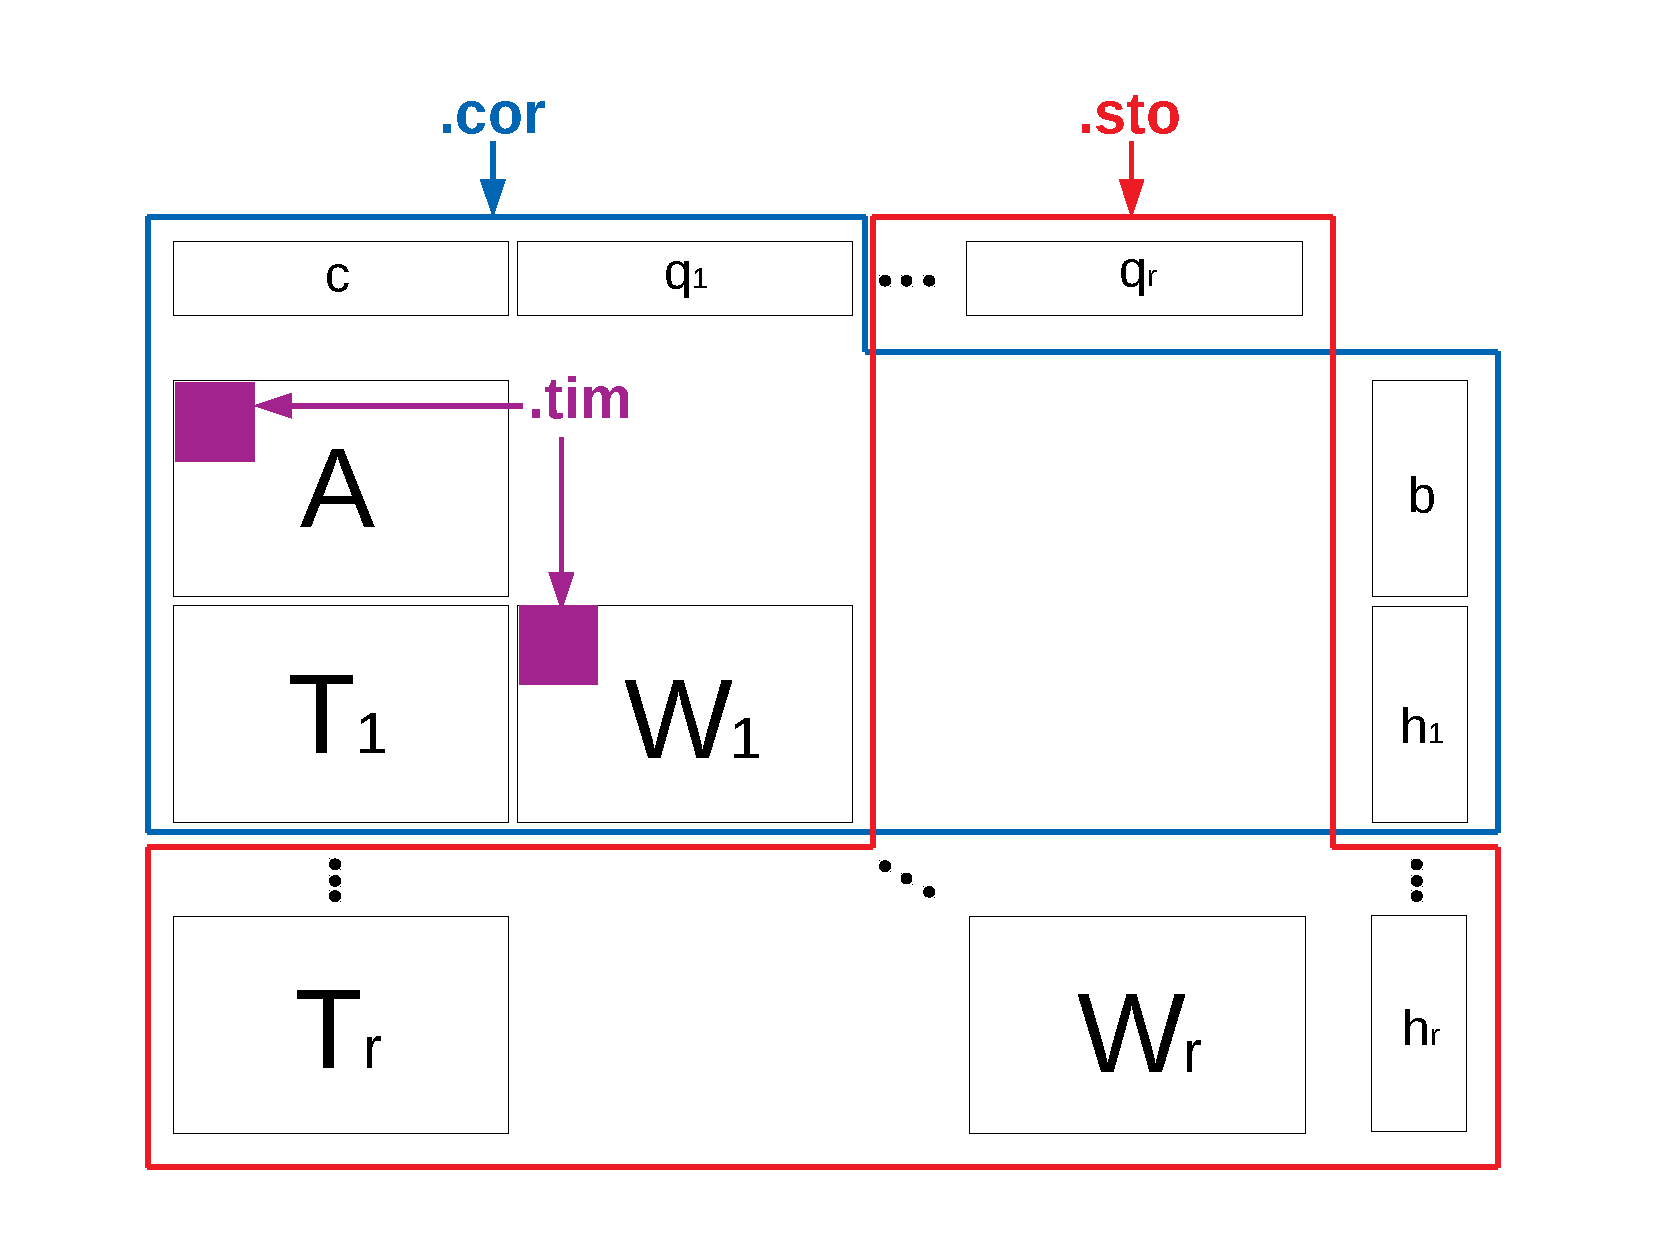
\includegraphics[width=\textwidth]{SMPS_description_slide}
\end{center}
\end{figure}
\end{frame}

\begin{frame}{\julia\ language}
\textbf{\footnote{\tiny Available at: \href{https://julialang.org /}{https://julialang.org/}}{Julia programming language} is a \textcolor{blue}{flexible dynamic language}, appropriate for \textcolor{blue}{scientific and numerical computing}, with \textcolor{blue}{performance} comparable to traditional statically-typed languages.} 
\begin{figure}
\begin{center}
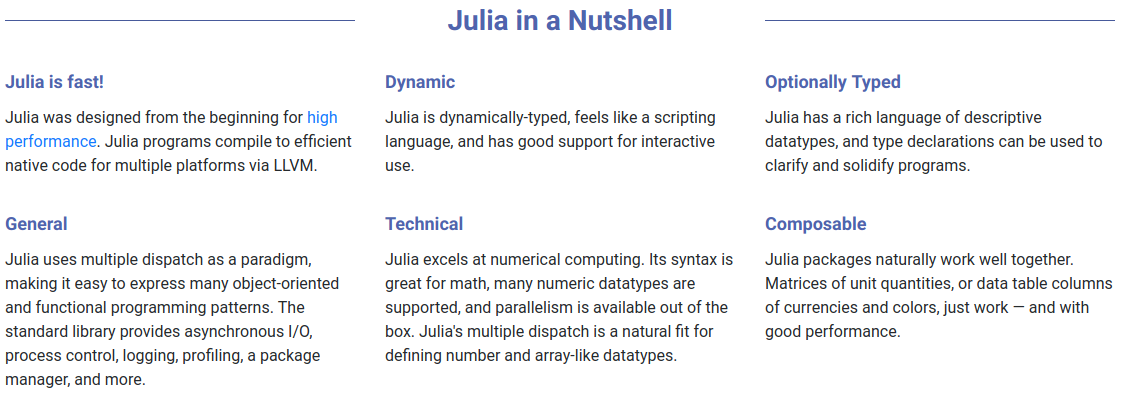
\includegraphics[width=\textwidth]{julia_nutshell}
\end{center}
\end{figure}	
\end{frame}

\begin{frame}{\structjump\ package}
\textbf{\footnote{\tiny Available at: \href{https://github.com/StructJuMP/StructJuMP.jl}{https://github.com/StructJuMP/StructJuMP.jl}}{\structjump} is a \julia\ package for modeling structured optimization models.}
\begin{itemize}
\item \textbf{\structjump} is an \textcolor{blue}{extension of \textbf{\jump} package}, a domain-specific modeling language for mathematical optimization embedded in \julia.
\begin{itemize}
\item \textbf{\jump} is generic, fast, and straightforward modeler.
\end{itemize}
\item \textbf{\structjump} provides a parallel algebraic modeling framework for \textcolor{blue}{block-structured optimization models} in \julia.
\item \textbf{\structjump} constructs a \textcolor{blue}{\textbf{\jumpmodel}-type object} that contains every information of an SIP instance.
\end{itemize}
\end{frame}

%	\begin{frame}{Modeling SIP using \structjump}
%	\begin{figure}[]
%		\centering
%		\begin{lstlisting}[frame=single,language=julia]
%		function DCAP(nR::Int, nN::Int, nT::Int, nS::Int, seed::Int=1)::JuMP.Model
%		
%		# set random seed (default=1)
%		srand(seed)
%		
%		# generate & store instance data
%		## sets
%		R = 1:nR
%		N = 1:nN
%		T = 1:nT
%		S = 1:nS
%		
%		## parameters
%		a = rand(nR, nT) * 5 + 5
%		b = rand(nR, nT) * 40 + 10
%		c = rand(nR, nN, nT, nS) * 5 + 5
%		c0 = rand(nN, nT, nS) * 500 + 500
%		d = rand(nN, nT, nS) + 0.5
%		Pr = ones(nS)/nS
%		
%		# construct a structured JuMP.Model
%		## declare an object
%		model = StructuredModel(num_scenarios = nS)
%		
%		## declare 1st stage components
%		@variable(model, x[i=R,t=T] >= 0)
%		@variable(model, u[i=R,t=T], Bin)
%		@objective(model, Min, sum(a[i,t]*x[i,t] + b[i,t]*u[i,t] for i in R for t in T))
%		@constraint(model, [i=R,t=T], x[i,t] - u[i,t] <= 0)
%		
%		## declare 2nd stage components
%		for s in S
%		sb = StructuredModel(parent=model, id = s, prob = Pr[s])
%		@variable(sb, y[i=R, j=N, t=T], Bin)
%		@variable(sb, z[j=N,t=T], Bin)
%		@objective(sb, Min, sum(c[i,j,t,s]*y[i,j,t] for i in R for j in N for t in T) + sum(c0[j,t,s]*z[j,t] for j in N for t in T))
%		@constraint(sb, [i=R, t=T], -sum(x[i,tau] for tau in 1:t) + sum(d[j,t,s]*y[i,j,t] for j in N) <= 0)
%		@constraint(sb, [j=N, t=T], sum(y[i,j,t] for i in R) + z[j,t] == 1)
%		end
%		
%		return model
%		end
%		\end{lstlisting}
%		\caption{An example of modeling SIP using \structjump: \texttt{DCAP\_model.jl}}\label{fig:DCAP_model.jl}
%	\end{figure}

%	\end{frame}

\section{Implementation of a Julia package: Siplib.jl}
\begin{frame}<beamer>{Contents}
\tableofcontents[currentsection,currentsubsection,hideothersubsections]
\end{frame}	

\begin{frame}{Core functionality of \siplibjl}
\textbf{Generating \smps\ files of SIP instance}:
\begin{figure}
\begin{center}
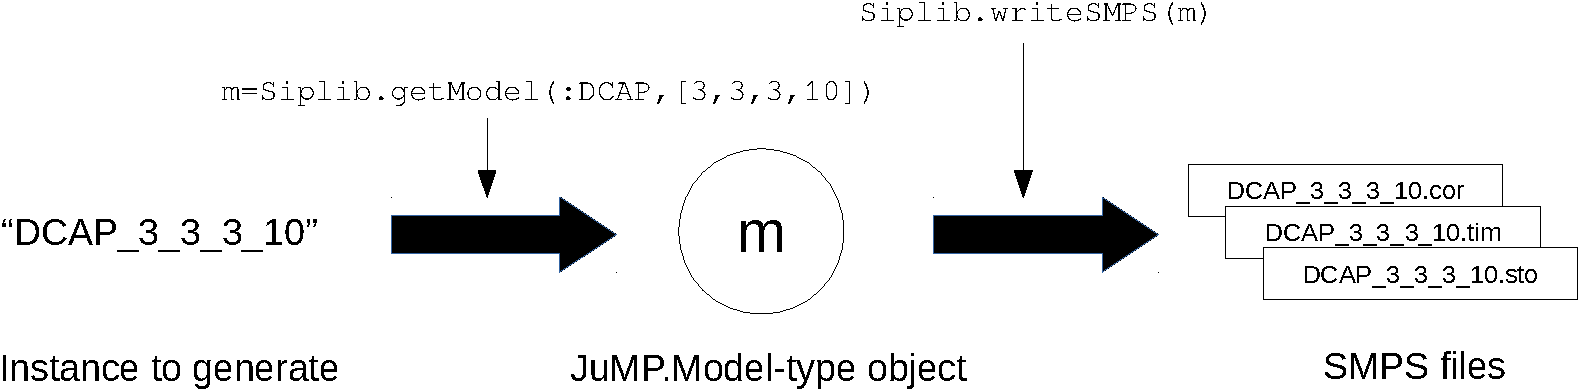
\includegraphics[width=\textwidth]{siplib_package}
\end{center}
\end{figure}	
\end{frame}

\begin{frame}{Problems available in \siplibtwo}
We implement \texttt{Julia} scripts for modeling 11 different problems from various sources and embed them into \siplibjl.
\ttiny
\begin{table}[H]
\centering
%\resizebox{}{!}{%
\label{table:problems}
\begin{tabular}{@{}llll@{}}
\toprule
Problem		  		  & Description                                                        & Main reference              \\ \midrule
\airlift\ & Airlift operations scheduling & Midler and Wollmer (1969)  \\
\cargo\ & Cargo network scheduling  & Mulvey and Ruszczy\`{n}ski (1995) \\
\chem\ & Design of batch chemical plants& Subrahmanyam et al. (1994) \\				
\dcap\         & \makecell[tl]{Dynamic capacity planning with stochastic\\ demand  }                  & Ahmed and Garcia (2003)                           \\
\mptsps\       & \makecell[tl]{Multi-path traveling salesman problem with\\ stochastic travel costs } & Tadei et al. (2017)                             \\
\phone\       & Telecommunication network planning & Sen et al. (2004)                            \\
\sdcp\ 	& Stochastic data center placement  & Kim et al. (2017) \\
\sizes\        & \makecell[tl]{Optimal product substitution with stochastic\\ demand}         & Jorjani et al. (1999)        \\
\smkp\		  & Stochastic multiple knapsack problem                               & Angulo et al. (2016)                           \\
\sslp\         & Stochastic server location problem                                 & Ntaimo and Sen (2005)                           \\
\suc\         & Stochastic unit commitment problem			               & Papavasiliou and Oren (2013)                        \\ \bottomrule
\end{tabular}%
\end{table}
\end{frame}

\begin{frame}{Problems available in \siplibtwo}
We parameterize the problems to let users tailor the instances and generate \smps\ files as they want.
\ttiny
\begin{table}[H]
\centering
%			\caption{Instance naming rules}
\label{table:naming_rule}
\resizebox{\textwidth}{!}{%
\begin{tabular}{@{}llp{0.6\textwidth}}
%		\begin{tabular}{@{}llp{3in}}
\toprule
Problem & Instance name                 & \multicolumn{1}{c}{Remark}                                                                    					      \\ \midrule
\airlift	& AIRLIFT\_$\mathcal{S}$& $\mathcal{S}$: number of scenarios\\
\cargo	& CARGO\_$\mathcal{S}$& $\mathcal{S}$: number of scenarios\\		
\chem	& CHEM\_$\mathcal{S}$& $\mathcal{S}$: number of scenarios\\				
\dcap\    & DCAP\_$R$\_$N$\_$T$\_$\mathcal{S}$    &   $R$: number of resources, $N$: number of tasks, $T$: number of time periods, $\mathcal{S}$: number of scenarios        \\
\mptsps\  & MPTSPs\_$d$\_$N$\_$\mathcal{S}$ &$d$: node distribution strategy, $N$: number of nodes, $\mathcal{S}$: number of scenarios\\
\phone	& PHONE\_$\mathcal{S}$& $\mathcal{S}$: number of scenarios\\
\sdcp\ & SDCP\_$k$\_$p$\_$d$\_$\mathcal{S}$ & $k$: maximum number of dispatchable loads, $p$: wind penetration level (\%), $d$: day type, $\mathcal{S}$: number of scenarios\\
\sizes\   & SIZES\_$\mathcal{S}$                            & $\mathcal{S}$: number of scenarios   															\\
\smkp\    &   SMKP\_$I$\_$\mathcal{S}$    &   $I$: number of types for item, $\mathcal{S}$: number of scenarios  													 \\
\sslp\    &  SSLP\_$I$\_$J$\_$\mathcal{S}$      &    $I$: number of clients, $J$: number of server locations, $\mathcal{S}$: number of scenarios                 				   \\
\suc\    & 	SUC\_$d$\_$\mathcal{S}$    &  $d$: day type, $\mathcal{S}$: number of scenarios                                                 						 \\ \bottomrule
\end{tabular}%
}
\end{table}
\end{frame}

\begin{frame}{Components of the problems}
We classify the problems based on their stage-wise variable types (continuous, binary, integer).		
\begin{table}[H]
\seven
\centering
%			\caption{Components of the problems}
\label{table:prob_class}
\begin{threeparttable}
\begin{tabular}{@{}lllll@{}}
\toprule
& \multicolumn{2}{c}{1st stage}                              				  	& \multicolumn{2}{c}{2nd stage}                             			        \\ \midrule
Problem 	     & Variable                    & Constraint                   	& Variable                    & Constraint                  				    \\ \midrule
\airlift\  & $\mathbb{I}$ & \texttt{IKN}& $\mathbb{C}$, $\mathbb{I}$ & \texttt{BIN}, \texttt{GEN}\\
\cargo\  & $\mathbb{I}$ & \texttt{IKN} & $\mathbb{C}$ & \texttt{GEN}\\		
\chem\  & $\mathbb{C}$, $\mathbb{I}$ & \texttt{VBD}, \texttt{GEN} & $\mathbb{C}$, $\mathbb{B}$ & \texttt{GEN}\\				
\dcap\     & $\mathbb{C}$, $\mathbb{B}$  & \texttt{VBD}                	& $\mathbb{B}$                & \texttt{PAR}, \texttt{M01} 			    		\\
\mptsps\   & $\mathbb{C}$, $\mathbb{B}$  & \texttt{PAR}, \texttt{GEN}		& $\mathbb{B}$                & \texttt{GEN}               						\\
\phone\  & $\mathbb{C}$ & \texttt{IVK} & $\mathbb{C}$, $\mathbb{I}$ & \texttt{GEN} \\			
\sdcp\ & $\mathbb{I}$ & \texttt{IKN}& $\mathbb{C}$ & \texttt{GEN}\\
\sizes\  & $\mathbb{I}$ 			   & \texttt{VBD}, \texttt{GEN} 	& $\mathbb{B}$, $\mathbb{I}$  & \texttt{IKN}             						\\
\smkp\   & $\mathbb{B}$                & \texttt{KNA}                	& $\mathbb{B}$                & \texttt{KNA}              						\\
\sslp\   & $\mathbb{B}$                & \texttt{IVK}, \texttt{GEN} 	& $\mathbb{C}$, $\mathbb{B}$  & \texttt{GEN}             						\\
\suc\   & $\mathbb{C}$, $\mathbb{B}$                 & \texttt{VBD}, \texttt{GEN}       	& $\mathbb{C}$, $\mathbb{B}$  &  \texttt{VBD}, \texttt{GEN}                                  					\\ \bottomrule
\end{tabular}
\end{threeparttable}
\end{table}
\vspace{-0.5cm}
\begin{itemize}
\item $\mathbb{C}$: continuous, $\mathbb{B}$: binary, $\mathbb{I}$: integer
\item Constraint type notation is adopted from \footnote{\tiny Available at: \href{http://miplib.zib.de/miplib2010.php}{http://miplib.zib.de/miplib2010.php}}{\miplib}.
\end{itemize}
\end{frame}

%	\begin{frame}[shrink=45]{Structure of the package}
%		\vspace{1cm}
%		\begin{minipage}[c][1.3\paperheight][c]{\textwidth}
%			\begin{figure} 
%				\begin{forest}
%					for tree={
%						font=\ttfamily,
%						grow'=0,
%						child anchor=west,
%						parent anchor=south,
%						anchor=west,
%						calign=first,
%						inner xsep=7pt,
%						edge path={
%							\noexpand\path [draw, \forestoption{edge}]
%							(!u.south west) +(7.5pt,0) |- (.child anchor) pic {folder} \forestoption{edge label};
%						},
%						% style for your file node 
%						file/.style={edge path={\noexpand\path [draw, \forestoption{edge}]
%								(!u.south west) +(7.5pt,0) |- (.child anchor) \forestoption{edge label};},
%							inner xsep=2pt,font=\small\ttfamily
%						},
%						before typesetting nodes={
%							if n=1
%							{insert before={[,phantom]}}
%							{}
%						},
%						fit=band,
%						before computing xy={l=15pt},
%					}  
%					[Siplib
%					[src
%					[problems
%					[AIRLIFT
%					[DATA
%					[numerical\_data.csv,file]
%					]
%					[AIRLIFT\_model.jl,file]
%					[AIRLIFT\_data.jl,file]
%					]
%					[CARGO
%					[CARGO\_model.jl,file]			
%					]
%					[$\ldots$]
%					]
%					[Siplib.jl,file]
%					[analyzer.jl,file]
%					[generator.jl,file]
%					[writer.jl,file]
%					[solver.jl,file]
%					[utility.jl,file]
%					[problem\_info.csv,file]
%					]
%					]
%					]
%				\end{forest}
%	%			\caption{Structure of the \julia\ package}\label{fig:siplibjl_structure}
%			\end{figure}
%		\end{minipage} 
%	\end{frame}

\section{Computational Experiments (work in progress)}
\begin{frame}<beamer>{Contents}
\tableofcontents[currentsection,currentsubsection,hideothersubsections]
\end{frame}	

\begin{frame}{Computing environment}
\begin{figure}
\begin{center}
\includegraphics[width=0.5\textwidth]{Bebop}
\end{center}
\end{figure}
%		\vspace{-1cm}
\begin{table}[H]
\centering
%			\caption{Experimental setting}
\label{table:experimental_setting}
\resizebox{\textwidth}{!}{%
\begin{tabular}{|l|l|}
\hline
\multirow{4}{*}{Computing facility} & \footnote{\tiny 1024-node computing cluster in Argonne National Lab (ANL):  \href{https://www.lcrc.anl.gov/systems/resources/bebop/}{https://www.lcrc.anl.gov/systems/resources/bebop/}}{\textit{Bebop}} with each node      \\
& - CPU: Intel Xeon Processor E5-2695 v4 (36 cores, 36 threads) \\
& - Clock speed: 2.10GHz (maximum 3.30GHz)                     \\
& - Memory:128GB (45MB Smart cache)                            \\ \hline
\multirow{2}{*}{Solver}                & General purpose MIP solver: CPLEX 12.8                                \\
& Open-source Dual Decomposition based SIP solver: DSP                                      \\ \hline
Multi-threading per instance                 & 36                                                           \\ \hline
Time limit per instance                            & 1 hours                                                      \\ \hline
\end{tabular}
}
\end{table}
\end{frame}

\begin{frame}{Computational report}
\begin{table}[H]
\centering
\caption{Computational report (template)}
\vspace{-0.5cm}
\label{table:computation_report}
\resizebox{\textwidth}{!}{%
\begin{tabular}{|l|ll|ll|l|l|l|}
\hline
& \multicolumn{2}{c|}{Objective value}                             & \multicolumn{2}{c|}{Optimality gap}                                & \multicolumn{1}{c|}{LP2-relax gap} & \multicolumn{1}{c|}{REVPI} & \multicolumn{1}{c|}{RVSS}  \\ \cline{2-8} 
\multicolumn{1}{|c|}{Instance} & \multicolumn{1}{c}{CPLEX  (SD)} & \multicolumn{1}{c|}{DSP  (SD)} & \multicolumn{1}{c}{CPLEX (time)} & \multicolumn{1}{c|}{DSP (time)} & \multicolumn{1}{c|}{CPLEX}         & \multicolumn{1}{c|}{CPLEX} & \multicolumn{1}{c|}{CPLEX} \\ \hline
AIRLIFT\_200                   &                                 &                                &                                  &                                 &                                    &                            &                            \\
AIRLIFT\_300                   &                                 &                                &                                  &                                 &                                    &                            &                            \\
AIRLIFT\_500                   &                                 &                                &                                  &                                 &                                    &                            &                            \\
AIRLIFT\_1000                  &                                 &                                &                                  &                                 &                                    &                            &                            \\ \hline
CARGO\_10                      &                                 &                                &                                  &                                 &                                    &                            &                            \\
CARGO\_50                      &                                 &                                &                                  &                                 &                                    &                            &                            \\
CARGO\_100                     &                                 &                                &                                  &                                 &                                    &                            &                            \\ \hline	
\end{tabular}%
}
\end{table}
\begin{itemize}
\item LP2-relax gap: Relative gap between the EF and LP-relaxation (2nd stage only)
\item REVPI: Relative Expected Value of Perfect Information
\item RVSS: Relative Value of Stochastic Solution
\end{itemize}
\end{frame}
%
%	\begin{frame}{Computational report}	
%		\begin{table}[H]
%			\eight
%			\centering
%			\caption{Gap definitions}
%			\vspace{-0.2cm}
%			\label{table:gap}
%			\begin{tabular}{lcc}
%				\hline
%				Gap   & Target to compare ($v$) & Reported value                                                        \\ \hline
%				Optimality gap (OG)   & $z$, $z_{LD}$    & \multirow{4}{*}{$\frac{|\hat{z}-v|}{|\hat{z}|+\epsilon}\times 100\%$} \\
%				LP2-relax gap (LG)   & $z_{LP2}$    &                                                                       \\
%				%		Duality gap (DG)   &      &                                                                       \\
%				Relative EVPI (REVPI) & $z_{WS}$     &                                                                       \\
%				Relative VSS (RVSS)  & $z_{EEV}$    &                                                                       \\ \hline
%			\end{tabular}
%		\end{table}
%	
%		\begin{table}[H]
%			\eight
%			\centering
%			\caption{Notations used to report computational result}
%			\vspace{-0.5cm}
%			\label{table:objective-notation}
%			\resizebox{\textwidth}{!}{%
%				\begin{threeparttable}
%					%		\begin{tabular}{@{}ll@{}}
%					\begin{tabular}{@{}lp{0.8\textwidth}}
%						\toprule
%						Notation  & \multicolumn{1}{c}{Meaning}                                                                                                                    \\ \midrule
%						$z$       & Objective value of the recourse problem  \\
%						$z_{LP2}$ & Objective value of RP with the second-stage only LP-relaxation                                       \\
%						$z_{LD}$  & Objective value of the Lagrangian dual problem of the recourse problem \\ 
%						$z_{EV}$ & Objective value of the expected value problem \\
%						$z_{EEV}$ & Objective value of RP using the first-stage solution of the expected value problem  \\
%						$z_s$ & Objective value of a single scenario problem given scenario $s$ \\
%						$z_{WS}$ & Averaged value of all single scenario problem objectives\\
%						$\sigma_{RP}$ & Standard deviation of the recourse problem\\
%						\bottomrule
%					\end{tabular}
%				\end{threeparttable}
%			}
%		\end{table}		
%	\end{frame}

\begin{frame}{}
\centering \Huge
\emph{Any suggestions are welcome!}
\end{frame}

\begin{frame}[noframenumbering]{Appendix: Deterministic Equivalent Form SIP}
\textbf{Example:} \dcap\ (dynamic capacity planning with stochastic demand)
\eight
\begin{subequations} \label{dcap:formulation}
\begin{align}
\textrm{(\dcap) }\textrm{min}\ &\sum_{t\in T}\sum_{i\in R}\left(\alpha_{it}x_{it}+\beta_{it}u_{it}\right)+\sum_{s\in\mathcal{S}}\PP(s)\sum_{t\in T}\sum_{i\in R\cup\{0\}}\sum_{j\in N}c_{ijt}^{s}y_{ijt}^s	\label{dcap:obj} \\
\textrm{s.t.}\ & x_{it}\le \textrm{M}u_{it},\quad\forall i\in R,\ \forall t\in T,	\label{dcap:b}\\
&\sum_{j\in N}d_{jt}^s y_{ijt}^s\le\sum_{\tau=1}^{t}x_{i\tau},\quad\forall i\in R,\ \forall t\in T,\ \forall s\in\mathcal{S},\label{dcap:c}\\
&\sum_{i\in R\cup \{0\}}y_{ijt}^s=1,\quad\forall j\in N,\ \forall t\in T,\ \forall s\in\mathcal{S}, \label{dcap:d} \\
&x_{it}\ge 0,\quad\forall i\in R,\ \forall t\in T,\label{dcap:e} \\
&u_{it}\in\{0,1\}, \quad\forall i\in R,\ \forall t\in T,\label{dcap:f}\\
&y_{ijt}^s\in\{0,1\},\quad\forall i\in R\cup\{0\},\ \forall j\in N,\ \forall t\in T,\ \forall s\in\mathcal{S}.\label{dcap:g}
\end{align}
\end{subequations}
\end{frame}

\begin{frame}[noframenumbering]{Appendix: Modeling an SIP using \structjump}
\textbf{Example:} \dcap (dynamic capacity planning with stochastic demand)
\begin{figure}
\centering
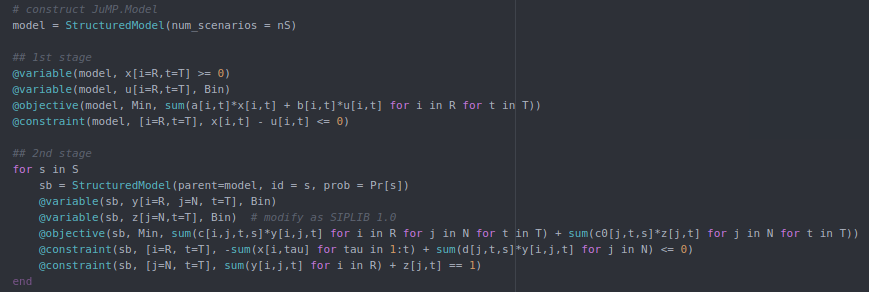
\includegraphics[width=\textwidth,keepaspectratio]{DCAP_modeling}
\end{figure}
\end{frame}

%
%	\begin{frame}
%	\frametitle{References}
%	\footnotesize{
%			\begin{thebibliography}{99} % Beamer does not support BibTeX so references must be nserted manually as below
%				\bibitem[Smith, 2012]{p1} John Smith (2012)
%				\newblock Title of the publication
%				\newblock \emph{Journal Name} 12(3), 45 -- 678.
%			\end{thebibliography}
%		}
%	\end{frame}


%	\begin{frame}{Backgrounds}
%		\emph{\textbf{Data Center}}
%		\begin{itemize}
%			\item A data center is a dedicated space where companies can keep and operate most of the \emph{ICT infrastructure} that supports their business
%			\item This would be the servers and storage equipment that \emph{run application software} and \emph{process and store data}
%		\end{itemize}
%		\begin{figure}
%			\begin{center}
%				\includegraphics[width=0.6\textwidth]{IDC}
%			\end{center}
%		\end{figure}
%	\end{frame}
%
%	\begin{frame}[shrink=10]{What is the problem?}
%	\emph{\textbf{Currently, most data centers are operating in wasteful manners}}
%		\begin{quote}
%			\small
%			\begin{tcolorbox}
%				\textbf{\textit{The Power of Efficiency to Cut Data Center Energy Waste}}\\ \\ \textit{\small 
%				$\cdots$NRDC has found that as much as 30 percent of a typical small office-based organization’s electricity bill may be due to \textcolor{red}{powering and cooling servers running around-the-clock even when performing little or no work}}$\cdots$\\
%				$\cdots$One of the largest remaining opportunities to save energy in data centers is \textcolor{blue}{to reduce electricity use when servers are unused, idle, or lightly used.} Decommissioning “zombie” (unused) servers, putting idle servers to a lower-power sleep mode$\cdots$\\
%				\begin{flushright}\textbf{Natural Resources Defense Council, \\June 30, 2016}\end{flushright}
%			\end{tcolorbox}
%		\end{quote}
%	\end{frame}
%
%	\begin{frame}{Research Goal}
%		\emph{\textbf{To develop an energy efficient operating algorithm for data centers that}}
%		\begin{itemize}
%			\item operates servers proportionally to demands
%			\item reflects the stochastic property of data center traffic
%			\item guarantees a certain service level
%			\item applies large-scale facility (many servers)
%		\end{itemize}
%	\end{frame}
%
%	\section{Mathematical Model}
%	
%	\begin{frame}<beamer>{Contents}
%		\tableofcontents[currentsection,currentsubsection,hideothersubsections]
%	\end{frame}
%
%	\begin{frame}{Problem Description}
%		\emph{\textbf{Assumptions}}
%		\begin{itemize}[<+->]
%			\item Applications are installed on servers in advance
%			\item Application $i$ requests are arriving by a \textcolor{blue}{stationary stochastic process} with rate $\lambda_i$ 
%			\item Each request brings $1/\mu_i$ amount of workload
%			\item Each server operates under the processor sharing (PS) discipline
%			\begin{itemize}
%				\item Each server is a \textcolor{blue}{$G/G/1/PS$} queue
%			\end{itemize}
%			\item Server $j$'s power function: $C_j(x_j)=K_j+\alpha_j {x_j}^n$ (Wierman et al.)
%		\end{itemize}
%		\vspace*{-0.2cm}
%		\begin{figure}
%			\centering
%			\fcolorbox{black}{white}
%			{
%				\includegraphics[width=\textwidth,height=0.35\textheight,keepaspectratio]{situation}
%			}
%		\end{figure}
%	\end{frame}
%	
%	\begin{frame}{Problem Description}
%		%\uncover<+->{\emph{\textbf{What to control}}}
%		\emph{\textbf{What to control (decision variables)}}
%		\begin{itemize}[<+->]
%			\item Workload routing ($y_{ij}$): amount of application $i$'s workload that are distributed to server $j$ 
%			\item Speed scaling ($x_j$): server $j$'s processing speed 
%		\end{itemize}
%		\vspace*{-0.2cm}
%		\begin{figure}
%			\centering
%			\fcolorbox{black}{white}
%			{
%				\includegraphics[width=\textwidth,height=0.35\textheight,keepaspectratio]{situation}
%			}
%		\end{figure}
%	\end{frame}
%	
%	\begin{frame}[shrink=0]{A Nonlinear Programming Formulation}
%	\vspace*{-0.5cm}
%		\begin{align}\texttt{}
%		\textrm{CP1}: \min &\sum_{j\in S}C_j(x_j)\\
%		\textrm{s.t.}& \nonumber \\
%		 &\sum_{i:i\in j}y_{ij} \leq x_j \quad \forall j\in S \\
%		&\sum_{j:i\in j}y_{ij}=w_i \quad \forall i\in A\\
%		&\gamma_j \leq x_{j}\leq \Gamma_j \quad\forall j\in S
%		\end{align}
%		%\vspace*{-0.5cm}
%		%\begin{itemize}
%			Objective (1): Minimize total power consumption\\
%			Constraint (2): Control server $j$'s speed\\% 서버 $j$로 분배되는 작업부하량(bits/s)은 \\$\qquad\qquad\quad$서버 j의 처리속도(bits/s)보다 적어야 함.\\
%			Constraint (3): Route application $i$'s workloads\\
%			Constraint (4): Restrict server $j$'s speed range
%		%\end{itemize}
%	\end{frame}
%
%	\begin{frame}{Response Time Consideration}
%		\textbf{\emph{Service Level Agreement (SLA)}}
%		\begin{itemize}
%			\item Constraint (Q): $\PP\{W_j \ge \delta_j\}\leq \epsilon_j\quad\forall j\in S$
%		\end{itemize}
%		\vspace{0.5cm}
%		\uncover<+(1)->{\textbf{\emph{In queueing theoritic perspective, constraint (2) may cause SLA violation}}}
%		\begin{itemize}[<+->]
%			\item (Recall) Constraint (2): $\sum_{i:i\in j}y_{ij} \leq x_j \quad \forall j\in S$
%			\item<+-> When $\rho=1$, $L=\lim_{t\to\infty} \EE[X(t)] = \infty$, then by Little's law $W=\infty$.       
%			\item<+-> Therefore, we should keep the server speed \emph{strictly} faster than $\sum_{i:i\in j}y_{ij}$.
%			\begin{itemize}
%				\item<.-> $\sum_{i:i\in j}y_{ij}+ \textcolor{blue}{\kappa_j} \leq x_j$ 
%				\item<.-> Which $\kappa_j$ is optimal?
%			\end{itemize}
%		\end{itemize}
%	\end{frame}
%
%	\begin{frame}{Response Time Consideration}
%		\textbf{\emph{Steady state approximations of LPS queues in heavy traffic (Zhang and Zwart, QUESTA, 2008)}}
%		\begin{itemize}
%			\item Using diffusion approximation, the steady state probabilities of $G/G/1/PS$ queue are derived
%		\end{itemize}
%		\uncover<+(1)->{\textbf{\emph{Approximation for the constraint (Q)}}}
%		\begin{itemize}[<+->]
%			\item<2-> From the result of Zhang and Zwart, $\PP\{W_j \ge \delta_j\}\approx \exp{\left( -\left(\frac{1+C_{s,j}^2}{C_{a,j}^2+C_{s,j}^2}\right) \left(\frac{x_j}{\sum_{i:i\in j}y_{ij}}-1\right) \left(\sum_{i:i\in j}\mu_i y_{ij}\right)\delta_j \right)}\leq \epsilon_j$
%			\begin{itemize}
%				\item<2-> $C_{s,j}$: Coefficient of variation of server $j$'s service time
%				\item<2-> $C_{a,j}$: Coefficient of variation of inter-arrivals time for server $j$
%			\end{itemize}
%		\end{itemize}
%		\uncover<+(1)->{\textbf{\emph{Modified constraint (2)}}}
%		\begin{itemize}[<+->]
%			\item $\left(\sum_{i:i\in j}y_{ij}\right)\left\{ \frac{\left(-\log{\epsilon_j}\right)\left(C_{a,j}^2+C_{s,j}^2\right)}{\left(\sum_{i:i\in j}\mu_i y_{ij}\right)\delta_j\left(1+C_{s,j}^2\right)}+1 \right\}\leq x_j\quad\forall j\in S\qquad (2')$ 
%		\end{itemize}
%	\end{frame}
%
%	\begin{frame}[label=lemma]{Response Time Consideration \hyperlink{proof}{\beamergotobutton}}
%		\textbf{\emph{Lemma for relaxing nonlinearity of constraint (2')}}
%		\begin{lemma}					
%		  \footnotesize
%		  %\normalsize
%		  Assuming that the routing of traffic is determined in a probabilistic way,
%		  \[
%			\left(\sum_{i:i\in j}y_{ij}\right)\left\{ \frac{\left(-\log{\epsilon_j}\right)\left(C_{a,j}^2+C_{s,j}^2\right)}{\left(\sum_{i:i\in j}\mu_i y_{ij}\right)\delta_j\left(1+C_{s,j}^2\right)}+1 \right\}\leq \sum_{i:i\in j}y_{ij} + \frac{  \left(-\log{\epsilon_j}\right) \max{(1,C_a^2)}  }{\mu_{\min}\delta_j},
%			\]\\
%			where $\mu_{\min}=\min_{i\in A}\mu_i$ and $C_a^2$ is the squared CV (SCV) of the inter-arrival times of aggregate requests from all applications.
%		\end{lemma}	
%	\end{frame}
%	
%	\begin{frame}{Modified Nonlinear Programming Formulation}
%		\begin{align}
%			\textrm{CP2}: \min &\sum_{j\in S}C_j(x_j) \tag{1}\\
%			\textrm{s.t.}& \nonumber\\
%			&\sum_{i:i\in j}y_{ij} +  \textcolor{blue}{\kappa_j} \leq x_j   \quad \forall j\in S \tag{2'}\\
%			&\sum_{j:i\in j}y_{ij}=w_i \quad \forall i\in A \tag{3}\\
%			&\gamma_j \leq x_{j}\leq \Gamma_j \quad\forall j\in S \tag{4}
%		\end{align}
%		where
%		\begin{displaymath}
%			\textcolor{blue}{\kappa_j =  \frac{  \left(-\log{\epsilon_j}\right) \max{(1,C_a^2)}  }{\mu_{\min}\delta_j}}
%		\end{displaymath}
%	\end{frame}
%
%	\section{Distributed Algorithm}
%	
%	\begin{frame}<beamer>{Contents}
%		\tableofcontents[currentsection,currentsubsection,hideothersubsections]
%	\end{frame}	
%
%	\begin{frame}[shrink=10,label=step]{Distributed Algorithm (Kelly et al.) \hyperlink{alg}{\beamergotobutton}}
%		\begin{enumerate}[<+->]
%			\item<1-> Introduce the constraint (2') into the objective using Lagrange multiplier \textcolor{blue}{$p_j$}.
%			\begin{align*}
%				&\min\sum_{j\in S}C_j(x_j)-\sum_{j\in S}\textcolor{blue}{p_j}\left(x_j-\sum_{i:i\in j}y_{ij}-\kappa_j\right)\\
%				&=\underbrace{\min\sum_{j\in S}\left[C_j(x_j)-\textcolor{blue}{p_j}(x_j-\kappa_j)\right]}_{\textrm{w.r.t. } x_j}+\underbrace{\min\sum_{j\in S}\sum_{i:i\in j}y_{ij}\textcolor{blue}{p_j}}_{\textrm{w.r.t. } y_{ij}}
%			\end{align*}
%			\item<2-> Separate the problem into two independent problems sharing \textcolor{blue}{$p_j$}.
%			%\vspace*{-0.5cm}
%			\begin{columns}<2->
%				\begin{column}{0.4\textwidth}
%					\begin{flushleft}
%						\underline{Server's speed scaling}
%						\begin{align*}
%							SP:\min_{x_j}&\sum_{j\in S}\left[C_j(x_j)-\textcolor{blue}{p_j}(x_j-\kappa_j)\right]\\
%							s.t.\textrm{ } &\gamma_j\le x_j\le \Gamma_j\quad\forall j\in S\\
%							\quad \\
%						\end{align*}
%					\end{flushleft}
%				\end{column}
%		
%				\begin{column}{0.4\textwidth}
%					\begin{flushleft}
%						\underline{Load balancer's workload routing}
%						\begin{align*}
%						LP1: \min_{y_{ij}}&\sum_{j\in S}\sum_{i:i\in j}y_{ij}\textcolor{blue}{p_j}\\
%						s.t. &\sum_{j:i\in j}y_{ij} = w_i \quad \forall i\in A \\
%						&\sum_{i:i\in j}y_{ij}\leq \Gamma_j \quad \forall j\in S
%						\end{align*}
%					\end{flushleft}
%				\end{column}
%			\end{columns} 
%			\saveenum
%		\end{enumerate}
%	\end{frame}
%
%	\begin{frame}{Distributed Algorithm (Kelly et al.) \hyperlink{alg}{\beamergotobutton}}
%		\begin{enumerate}
%			\resume
%			\item Update each server's $x_j$, $p_j$ values using \textit{gradient method}.
%			\begin{itemize}
%				\item Server speed ($x_j$)
%				\begin{align*}
%				&\dot{x}_j^{(k)} = \left\{ 
%				\begin{array}{ll}
%				\max\left(0, p_j^{(k)}-C_j'\left(x_j^{(k)}\right)\right) & \textrm{if $x_j^{(k)} = \gamma_j$}, \\
%				p_j^{(k)}-C_j'\left(x_j^{(k)}\right) & \textrm{if $x_j^{(k)} \in (\gamma_j,\Gamma_j)$},\\
%				\min\left(0, p_j^{(k)}-C_j'\left(x_j^{(k)}\right)\right) & \textrm{if $x_j^{(k)} = \Gamma_j.$}
%				\end{array} \right.  \\
%				&x_j^{(k+1)}=x_j^{(k)}+\nu_j^{(k)}\dot{x}_j^{(k)}.
%				\end{align*}
%				\item Lagrange multiplier ($p_j$)
%				\begin{align*}
%					&\dot{p}_j^{(k)} = \left\{ 
%										\begin{array}{ll}
%											\kappa_j+\sum_{i:i\in j}y_{ij}^{(k)}-x_j^{(k)} & \textrm{if $p_j^{(k)} \geq 0$}, \\
%											\max\left(0, \kappa_j+\sum_{i:i\in j}y_{ij}^{(k)}-x_j^{(k)}\right) & \textrm{otherwise.}
%										\end{array} \right .  \\
%					&p_j^{(k+1)}=p_j^{(k)}+\eta_j^{(k)}\dot{p}_j^{(k)}.
%				\end{align*}
%			\end{itemize}
%			\saveenum
%		\end{enumerate}
%	\end{frame}
%	
%	\begin{frame}{Distributed Algorithm (Kelly et al.) \hyperlink{alg}{\beamergotobutton}}
%		\begin{enumerate}
%			\resume
%			\item Formulate a problem (LP2) incorporating $x_j^{(k+1)}, p_j^{(k+1)}$ and update $y_{ij}$.
%			\begin{align*}
%				LP2: \min_{y_{ij}^{(k+1)}}&\sum_{j\in S}\sum_{i:i\in j}p_j^{(k+1)}y_{ij}^{(k+1)}\\
%				s.t. &\sum_{j:i\in j}y_{ij}^{(k+1)} = w_i \quad \forall i\in A \\
%				&\sum_{i:i\in j}y_{ij}^{(k+1)}\leq \Gamma_j \quad \forall j\in S
%			\end{align*}
%			\item Iterate steps 3 and 4 until convergence.
%		\end{enumerate}
%	\end{frame}
%
%	\section{Experiments}
%	
%	\begin{frame}<beamer>{Contents}
%		\tableofcontents[currentsection,currentsubsection,hideothersubsections]
%	\end{frame}
%	
%	\begin{frame}{Design of Experiments ($G/G/1/PS$)}
%		\begin{table}
%			\caption{Server Parameters}
%			\vspace{-0.2cm}
%			\begin{adjustbox}{width=\textwidth}
%				\begin{tabular}{|c|c|c|c|c|c|c|c|c|c|c|}
%					\hline 
%					Server $(j)$ & Speed LB ($\gamma_j$) & Speed UB ($\Gamma_j$) & $K_j$ & $\alpha_j$ & $n$ & $\delta_j$ & $\epsilon_j$ & $x_j^{(0)}$ & $p_j^{(0)}$ & Apps \\ 
%					\hline 
%					1 & 5 & 100 & 150 & 0.3333 & 3 & 3 & 0.001 & 100 & 1000 & 1 \\ 
%					\hline 
%					2 & 7 & 102 & 250 & 0.2 & 3 & 3 & 0.001 & 102 & 2000 & 1 \\ 
%					\hline 
%					3 & 6 & 99 & 220 & 1 & 3 & 3 & 0.001 & 99 & 3000 & 1,2 \\ 
%					\hline 
%					4 & 5 & 105 & 150 & 0.6667 & 3 & 3 & 0.001 & 105 & 1000& 1,2,3  \\ 
%					\hline 
%					5 & 7 & 100 & 300 & 0.8 & 3 & 3 & 0.001 & 100 & 2000 & 2,3 \\ 
%					\hline 
%					6 & 8 & 102 & 350 & 0.4 & 3 & 3 & 0.001 & 102 & 3000 &  2,3\\ 
%					\hline 
%					7 & 6 & 100 & 220 & 0.4286 & 3 & 3 & 0.001 & 100 & 1000 & 3\\ 
%					\hline 
%					8 & 7 & 105 & 350 & 0.5 & 3 & 3 & 0.001 & 105 & 2000 & 4,5 \\ 
%					\hline 
%					9 & 8 & 102 & 400 & 0.6 & 3 & 3 & 0.001 & 102 & 3000 & 4,5 \\ 
%					\hline 
%					10 & 10 & 105 & 700 & 0.4444 & 3 & 3 & 0.001 & 105 & 1000 & 5 \\ 
%					\hline 
%				\end{tabular}
%			\end{adjustbox}
%		\end{table}
%		\vspace*{-0.2cm}
%		\begin{itemize}
%			\item Power function of server $j$: $C_j(x)=K_j+\alpha_j x^n$
%			\item Service level constraint: $\PP\left\{W_j\ge\delta_j \right\}\le\epsilon_j$ 
%				\begin{itemize}
%					\item We set $\PP\left\{W_j\ge 3 \right\}\le 0.001$ for all servers
%				\end{itemize}
%			\item Regular update interval: 0.01 sec
%			\item Terminal criterion: 200,000 departures	 
%		\end{itemize}
%	\end{frame}
%	
%	\begin{frame}{Design of Experiments ($G/G/1/PS$)}
%		\begin{table}
%			\caption{User Request Parameters}
%			\vspace{-0.5cm}
%			\begin{adjustbox}{width=\textwidth}
%				\begin{tabular}{|c|c|c|c|c|c|c|}
%					\hline
%					\multirow{2}{*}{Application ($i$)} & \multicolumn{3}{c|}{Inter-arrival Time ($X_i$)}            & \multicolumn{3}{c|}{Workload ($Y_i$)} \\ \cline{2-7} 
%					& Distribution          & Mean $(1/\lambda_i)$ & SCV & Distribution         & Mean $(1/\mu_i)$  & SCV \\ \hline
%					1                             & Lognormal   & 0.25              & 2    & Lognormal  & 5              & 1.5  \\ \hline
%					2                             & Lognormal   & 0.5               & 1.5  & Lognormal  & 10             & 2    \\ \hline
%					3                             & Exponential & 0.25              & 1    & Lognormal  & 5              & 1    \\ \hline
%					4                             & Lognormal   & 0.1               & 0.8  & Lognormal  & 2              & 0.8  \\ \hline
%					5                             & Lognormal   & 0.2               & 2    & Lognormal  & 3              & 0.5  \\ \hline
%				\end{tabular}
%			\end{adjustbox}
%		\end{table}
%	\end{frame}
%	
%	\begin{frame}{Result ($G/G/1/PS$ without buffer, $\kappa_j=0.0$)}
%		\begin{figure}
%			\centering
%			\includegraphics[width=\textwidth,keepaspectratio]{stationary_without_kappa}
%		\end{figure}
%	\end{frame}
%
%	\begin{frame}{Result ($G/G/1/PS$ without buffer, $\kappa_j=0.0$)}
%		\begin{center}
%			Constraint (Q): $\PP\left\{W_j\ge 3 \right\}\le 0.001$
%			\vspace{1cm}
%			\begin{adjustbox}{width=0.5\textwidth}
%				\begin{tabular}{|c|c|}
%					\hline 
%					Server ($j$) & $\PP\left\{W_j\ge\delta_j\right\}$ \\ 
%					\hline 
%					1 & 0.0395\\ 
%					\hline 
%					2 & 0.0365 \\ 
%					\hline 
%					3 & 0.0032 \\ 
%					\hline 
%					4 & 0.0321 \\ 
%					\hline 
%					5 & 0.0084 \\ 
%					\hline 
%					6 & 0.0294 \\ 
%					\hline 
%					7 & 0.0293 \\ 
%					\hline 
%					8 & 0.0629 \\ 
%					\hline 
%					9 & 0.0631 \\ 
%					\hline 
%					10 & 0.0369 \\ 
%					\hline 
%				\end{tabular}
%			\end{adjustbox}
%		\end{center}
%	\end{frame}
%	
%	\begin{frame}{Result ($G/G/1/PS$ with buffer, $\kappa_j=30.3941$)}
%		\begin{figure}
%			\centering
%			\includegraphics[width=\textwidth,keepaspectratio]{stationary_with_kappa}
%		\end{figure}
%	\end{frame}
%	
%	\begin{frame}{Result ($G/G/1/PS$ with buffer, $\kappa_j=30.3941$)}
%		\begin{center}
%			Constraint (Q): $\PP\left\{W_j\ge 3 \right\}\le 0.001$
%			\vspace{1cm}
%			\begin{adjustbox}{width=0.5\textwidth}
%				\begin{tabular}{|c|c|}
%					\hline 
%					Server ($j$) & $\PP\left\{W_j\ge\delta_j\right\}$ \\ 
%					\hline 
%					1 & 0.0\\ 
%					\hline 
%					2 & 0.0 \\ 
%					\hline 
%					3 & 0.0 \\ 
%					\hline 
%					4 & 0.0 \\ 
%					\hline 
%					5 & 0.0 \\ 
%					\hline 
%					6 & 0.00009 \\ 
%					\hline 
%					7 & 0.0 \\ 
%					\hline 
%					8 & 0.0 \\ 
%					\hline 
%					9 & 0.0 \\ 
%					\hline 
%					10 & 0.0 \\ 
%					\hline 
%				\end{tabular} 
%			\end{adjustbox}
%		\end{center}
%	\end{frame}
%
%	\section{Nonstationary Case}
%	
%	\begin{frame}<beamer>{Contents}
%		\tableofcontents[currentsection,currentsubsection,hideothersubsections]
%	\end{frame}
%	
%	\begin{frame}{Stationary$\to$Nonstationary}
%		\begin{itemize}
%			\item In real, data center traffic is nonstationary stochastic process with time-varying arrival rate
%			\item We need to modify the buffer $\kappa_j$ derived from assuming stationary processes
%		\end{itemize}
%%		\begin{columns}%[onlytextwidth]
%%			\begin{column}{0.5\textwidth}
%%				\begin{figure}
%%					\centering
%%					\includegraphics[width=0.8\textwidth]{slowly_varying}					
%%				\end{figure}
%%			\end{column}
%%			\hspace*{-1cm}
%%			\begin{column}{0.5\textwidth}
%%				\begin{figure}
%%					\centering
%%					\includegraphics[width=0.8\textwidth]{slowly_varying_with_big_spike}					
%%				\end{figure}
%%			\end{column}
%%		\end{columns}
%		\vspace{-0.5cm}
%		\begin{figure}
%			\centering
%			\subfloat[][Slowly varying]
%			{
%				\centering\includegraphics[width=0.45\linewidth]{slowly_varying}
%			}
%			\hspace{0.0cm}
%			\subfloat[][Slowly varying with spike]
%			{
%				\centering\includegraphics[width=0.45\linewidth]{slowly_varying_with_big_spike}
%			}
%			\vspace{0.4cm}
%			\caption{Real data center traffic (Gandhi et al.)}
%			%\label{data3}
%		\end{figure}
%	\end{frame}
%	
%	\begin{frame}{Majorizing piecewise constant rate function}
%		\begin{itemize}[<+->]
%			\item \textbf{Assumption:} Application $i$ requests are arriving by a \textcolor{blue}{nonstationary stochastic process} with rate function $\lambda_i(t)=a_i+b_i\sin{\left(\frac{\pi t}{c_i}\right)}$.\\
%			\item \textbf{Idea:} Divide $\lambda_i(t)$ into $N$ intervals. Regard the arrival process on each interval $T_n$ as a stationary process with rate $\max_{t\in{T_n}}{\lambda_i(t)}$. Then, we can decide the \textcolor{blue}{upper bound} of $\kappa_j$ at each interval. 
%		\end{itemize}
%		\begin{figure}
%			\centering
%			\includegraphics[width=0.8\textwidth,keepaspectratio]{rate}
%		\end{figure}
%	\end{frame}
%	
%	\begin{frame}{A Special Case: Nonstationary Poisson Process (NSPP)}
%		\begin{itemize}[<+->]
%			\item When all the arrival processes are NSPP, aggregated SCV is 1 for any time interval $T_n$, for $n=1,\dots,N$.
%			\begin{align*}
%				C_a^2(t) =\sum_{i\in A}\frac{\lambda_i(t)}{\sum_{i\in A}\lambda_i(t)}SCV(X_i(t))=1, \textrm{for $t\in T_n$}
%			\end{align*}
%			\begin{itemize}
%				\item<.-> $X_i(t)$: App $i$'s interarrival time on interval $T_n$
%				\item<.-> $X_i(t)\sim Exponential\left(\max_{\tau\in T_n}{\lambda_i(\tau)}\right)$
%			\end{itemize}
%			\item Therefore,
%			\begin{displaymath}
%			\kappa_j(t) =  \frac{  \left(-\log{\epsilon_j}\right) \max{(1,C_a^2(t))}  }{\mu_{\min}\delta_j}=\textcolor{blue}{-\frac{\log{\epsilon_j}  }{\mu_{\min}\delta_j}}\quad\forall j\in S,\forall t
%			\end{displaymath}
%		\end{itemize}
%	\end{frame}
%	
%	\begin{frame}{Design of Experiments}
%		\begin{table}[H]
%		\caption{NSPP Parameter}
%		\begin{center}
%			%\begin{adjustbox}{width=\textwidth}
%			\begin{tabular}{|c|c|}
%				\hline 
%				App ($i$) & Rate function $\left(\lambda_i(t)\right)$ \\ 
%				\hline 
%				1 & $4-3sin\left(\frac{\pi t}{1000}\right)$ \\ 
%				\hline 
%				2 & $2-1.5sin\left(\frac{\pi t}{1000}\right)$ \\ 
%				\hline 
%				3 & $4-2.5sin\left(\frac{\pi t}{1000}\right)$ \\ 
%				\hline 
%				4 & $10-5sin\left(\frac{\pi t}{1000}\right)$ \\ 
%				\hline 
%				5 & $5-4sin\left(\frac{\pi t}{1000}\right)$  \\ 
%				\hline 
%			\end{tabular}
%			%\end{adjustbox}
%
%		\end{center}
%	\end{table}
%	\end{frame}
%
%	\begin{frame}{Result ($M_t/G/1/PS$ without buffer, $\kappa_j=0.0$)}
%		\begin{figure}
%			\centering
%			\includegraphics[width=\textwidth,keepaspectratio]{nonstationary_without_kappa}
%		\end{figure}
%	\end{frame}
%
%	\begin{frame}{Result ($M_t/G/1/PS$ without buffer, $\kappa_j=0.0$)}
%		\begin{center}
%			Constraint (Q): $\PP\left\{W_j\ge 3 \right\}\le 0.001$
%			\vspace{1cm}
%			\begin{adjustbox}{width=0.5\textwidth}
%				\begin{tabular}{|c|c|}
%					\hline 
%					Server ($j$) & $\PP\left\{W_j\ge\delta_j\right\}$ \\ 
%					\hline 
%					1 & 0.0595 \\ 
%					\hline 
%					2 & 0.0553 \\ 
%					\hline 
%					3 & 0.0089 \\ 
%					\hline 
%					4 & 0.0331 \\ 
%					\hline 
%					5 & 0.0159 \\ 
%					\hline 
%					6 & 0.0433 \\ 
%					\hline 
%					7 & 0.0511 \\ 
%					\hline 
%					8 & 0.0524 \\ 
%					\hline 
%					9 & 0.0502 \\ 
%					\hline 
%					10 & 0.0468 \\ 
%					\hline 
%				\end{tabular} 
%			\end{adjustbox}
%		\end{center}
%	\end{frame}
%
%	\begin{frame}{Result ($M_t/G/1/PS$ with buffer, $\kappa_j=23.0259$)}
%		\begin{figure}
%			\centering
%			\includegraphics[width=\textwidth,keepaspectratio]{nonstationary_with_kappa}
%		\end{figure}
%	\end{frame}
%
%	\begin{frame}{Result ($M_t/G/1/PS$ with buffer, $\kappa_j=23.0259$)}
%		\begin{center}
%			Constraint (Q): $\PP\left\{W_j\ge 3 \right\}\le 0.001$
%			\vspace{1cm}
%			\begin{adjustbox}{width=0.5\textwidth}
%				\begin{tabular}{|c|c|}
%					\hline 
%					Server ($j$) & $\PP\left\{W_j\ge\delta_j\right\}$ \\ 
%					\hline 
%					1 & 0.00 \\ 
%					\hline 
%					2 & 0.00 \\ 
%					\hline 
%					3 & 0.00 \\ 
%					\hline 
%					4 & 0.00 \\ 
%					\hline 
%					5 & 0.00 \\ 
%					\hline 
%					6 & 0.00 \\ 
%					\hline 
%					7 & 0.00 \\ 
%					\hline 
%					8 & 0.00 \\ 
%					\hline 
%					9 & 0.00 \\ 
%					\hline 
%					10 & 0.00 \\ 
%					\hline 
%				\end{tabular} 
%			\end{adjustbox}
%		\end{center}
%	\end{frame}
%	\section{Conclusion}
%	
%	\begin{frame}<beamer>{Contents}
%	\tableofcontents[currentsection,currentsubsection,hideothersubsections]
%	\end{frame}
%
%	\begin{frame}{Conclusion and Future Plan}
%		\emph{\textbf{Conclusion}}
%		\begin{itemize}
%			\item Keep the service level in terms of \textcolor{blue}{tail probability of delay} rather than mean response time
%			\item Resolve large-scale by introducing the \textcolor{blue}{distributed algorithm}
%			\item $\kappa_j$ can be fixed constant when arrival processes are all NSPP
%		\end{itemize}
%		\vspace{0.5cm}
%		\uncover<+(1)->{\emph{\textbf{Future Plan}}}	
%		\begin{itemize}[<+->]
%			\item<+-> Full extension to $G_t/G/1/PS$ or $G_t/G_t/1/PS$
%			\begin{itemize}
%				\item<.-> currently we are working on the performance measures of $G_t/G_t/1/PS$
%			\end{itemize}
%		\end{itemize}	
%	\end{frame}
%	
%	\begin{frame}{}
%	\centering \Huge
%	\emph{Thank You}
%	\end{frame}
%	
%	\begin{frame}[shrink=20,noframenumbering,label=proof]{Appendix: Proof of Lemma \hyperlink{lemma}{\beamerreturnbutton}}
%		\begin{lemma}					
%			\footnotesize
%			%\normalsize
%			Assuming that the routing of traffic is determined in a probabilistic way,
%			\[
%			\left(\sum_{i:i\in j}y_{ij}\right)\left\{ \frac{\left(-\log{\epsilon_j}\right)\left(C_{a,j}^2+C_{s,j}^2\right)}{\left(\sum_{i:i\in j}\mu_i y_{ij}\right)\delta_j\left(1+C_{s,j}^2\right)}+1 \right\}\leq \sum_{i:i\in j}y_{ij} + \frac{  \left(-\log{\epsilon_j}\right) \max{(1,C_a^2)}  }{\mu_{\min}\delta_j},
%			\]\\
%			where $\mu_{\min}=\min_{i\in A}\mu_i$ and $C_a^2$ is the squared CV (SCV) of the inter-arrival times of aggregate requests from all applications.
%		\end{lemma}	
%		\begin{proof}
%			\begin{align}
%				C_{a,j}^2 \ge 1\Rightarrow C_{a,j}^2\ge\frac{C_{a,j}^2+C_{s,j}^2}{1+C_{s,j}^2} \\
%				\max(1,C_a^2)\ge C_{a,j}^2 \quad\textrm{by Whitt (1983)}\\
%				\frac{\sum_{i:i\in j}y_{ij}}{\sum_{i:i\in j}\mu_i y_{ij}} \le \frac{\sum_{i:i\in j}y_{ij}}{\sum_{i:i\in j}\mu_{\min} y_{ij}} = \frac{1}{\mu_{\min}} 
%			\end{align}
%			Equations (1)-(3) imply the lemma.
%		\end{proof}
%	\end{frame}
%
%	\begin{frame}[noframenumbering,label=alg]{Appendix: Optimality of the distributed algorithm \hyperlink{step}{\beamerreturnbutton}}
%		\emph{\textbf{Optimal solutions from a solver}}
%		\begin{figure}
%			\centering
%			\includegraphics[width=0.5\textwidth,keepaspectratio]{solver}
%		\end{figure}
%	\end{frame}
%
%	\begin{frame}[noframenumbering]{Appendix: Optimality of the distributed algorithm \hyperlink{step}{\beamerreturnbutton}}
%	\emph{\textbf{Result from the distributed algorithm}}
%		\begin{figure}
%			\centering
%			\includegraphics[width=0.75\textwidth,keepaspectratio]{Energy_consumption}
%		\end{figure}
%	\end{frame}
%
%	\begin{frame}[noframenumbering]{Appendix: Optimality of the distributed algorithm \hyperlink{step}{\beamerreturnbutton}}
%	\emph{\textbf{Result from the distributed algorithm}}
%	\vspace*{-0.3cm}
%		\begin{figure}
%			\centering
%			\includegraphics[width=0.8\textwidth,keepaspectratio]{Instantaneous_server_speeds}
%		\end{figure}
%	\end{frame}
\end{document}